\documentclass{standalone}

% ==== Essential Packages ====
\usepackage{tikz}
\usepackage{amsmath}
\usepackage{xcolor}
\usepackage{physics}
\usepackage{siunitx}
\usepackage{graphicx}
\usepackage{booktabs}
\usepackage{setspace}
\usepackage[font=small,labelfont=bf]{caption}
\usepackage[absolute,overlay]{textpos}
\usepackage{transparent}
\usepackage[subrefformat=parens,labelformat=parens]{subcaption}
\usepackage{shadowtext}
\usepackage{colortbl}
\usepackage[most]{tcolorbox}

% ==== TikZ Libraries ====
\usetikzlibrary{arrows.meta, decorations.pathreplacing, backgrounds, positioning, calc, shapes.geometric, decorations.pathmorphing}

% ==== Custom Colors ====
\definecolor{softyellow}{HTML}{F2D648}
\definecolor{dustyblue}{HTML}{9EB9D4}
\definecolor{berkeleyblue}{RGB}{0,50,98}
\definecolor{berkeleygold}{RGB}{253,181,21}
\definecolor{berkeleylight}{RGB}{198,217,241}
\definecolor{chalcogen}{RGB}{218,165,32}
\definecolor{metal}{RGB}{100,149,237}
\definecolor{tablegray}{gray}{0.95}
\definecolor{methodblue}{RGB}{100,120,180}
\definecolor{colgold}{RGB}{253,235,150} % very light gold tone

% ==== Custom tcolorbox ====
\newtcolorbox{rankingblock}[1]{
  colback=colgold,        % Background color
  colframe=berkeleyblue,  % Border color
  boxrule=0.4pt,
  arc=1mm,
  fontupper=\scriptsize,
  title=#1
}

\begin{document}

\begin{columns}[T]
  \column{0.5\textwidth}
  
  % Panel 1: Band Gap Modulation - Shortened text
  \begin{tcolorbox}[
    enhanced,
    colback=berkeleyblue!10,
    colframe=berkeleyblue,
    boxrule=0.8pt,
    arc=1mm,
    title={\textbf{Band Gap Engineering}},
    fonttitle=\small\bfseries,
    left=6pt, right=6pt,
    top=4pt, bottom=4pt
  ]
    \begin{itemize}\footnotesize\setlength{\itemsep}{0.3em}
      \item Compression ($C$) → Band gap tuning
      \item Non-monotonic $E_g(C)$ relationship
    \end{itemize}
    
    \begin{center}
      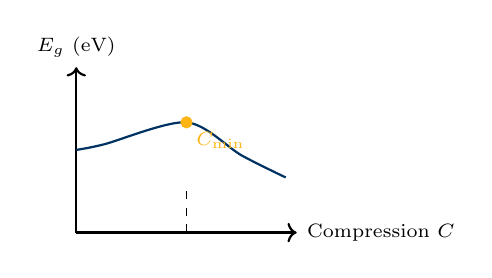
\begin{tikzpicture}[scale=0.7]
        % Axes
        \draw[->, thick] (0,0) -- (4,0) node[right, font=\scriptsize] {Compression $C$};
        \draw[->, thick] (0,0) -- (0,3) node[above, font=\scriptsize] {$E_g$ (eV)};
        
        % Band gap vs compression curve
        \draw[thick, berkeleyblue] plot[smooth] coordinates 
          {(0,1.5) (0.5,1.6) (2,2) (3,1.4) (3.8,1)};
          
        % Critical points
        \filldraw[berkeleygold] (2,2) circle (0.1) node[below right, font=\scriptsize] {$C_{\text{min}}$};
        \draw[dashed] (2,0) -- (2,0.8);
      \end{tikzpicture}
    \end{center}
  \end{tcolorbox}
  
  \column{0.5\textwidth}
  
  % Panel 2: Anisotropic Flattening - Shortened text
  \begin{tcolorbox}[
    enhanced,
    colback=berkeleygold!10,
    colframe=berkeleygold,
    boxrule=0.8pt,
    arc=1mm,
    title={\textbf{Anisotropic Behavior}},
    fonttitle=\small\bfseries,
    left=6pt, right=6pt,
    top=4pt, bottom=4pt
  ]
    \begin{itemize}\footnotesize\setlength{\itemsep}{0.3em}
      \item Flat along $k_y$ ($\overline{\Gamma\text{Y}}$)
      \item Partly flat along $k_x$ ($\overline{\Gamma\text{X}}$, $\overline{\text{Y}\text{S}}$)
    \end{itemize}
    
    \begin{center}
      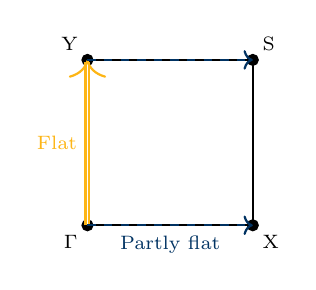
\begin{tikzpicture}[scale=0.7]
        % BZ with high-symmetry points
        \draw[thick] (0,0) rectangle (3,3);
        \filldraw (0,0) circle (0.1) node[below left, font=\scriptsize] {$\Gamma$};
        \filldraw (3,0) circle (0.1) node[below right, font=\scriptsize] {X};
        \filldraw (3,3) circle (0.1) node[above right, font=\scriptsize] {S};
        \filldraw (0,3) circle (0.1) node[above left, font=\scriptsize] {Y};
        
        % Flat direction indicators
        \draw[->, thick, berkeleygold, double] (0,0) -- (0,3) node[midway, left, font=\scriptsize] {Flat};
        \draw[->, thick, berkeleyblue, dashed] (0,0) -- (3,0) node[midway, below, font=\scriptsize] {Partly flat};
        \draw[->, thick, berkeleyblue, dashed] (0,3) -- (3,3);
      \end{tikzpicture}
    \end{center}
  \end{tcolorbox}
\end{columns}

\vspace{0.3cm}

% Summary panel at bottom - Condensed insights
\begin{tcolorbox}[
  enhanced,
  colback=white,
  colframe=berkeleyblue,
  boxrule=1pt,
  left=6pt, right=6pt,
  top=4pt, bottom=4pt
]
\begin{columns}[T]
  \column{0.48\textwidth}
  \scriptsize
  \textbf{Insight 1:} Compression tunes band gap without changing material composition.
  
  \column{0.48\textwidth}
  \scriptsize
  \textbf{Insight 2:} Anisotropic flattening creates direction-dependent transport channels.
\end{columns}

\end{document}
